\chapter{Background}


\section{Organization of the genome}

In Eukaryotes hereditary information is stored as DNA in the cell nucleus. Genomic DNA is transcribed and replicated. For example, if stretched into a single thread, human DNA is around 2 meters long and must be compacted into a microscopic nucleus. Therefore, multiple levels of organization are applied, starting from DNA helix and histone proteins and ending with chromosomes and their territories in the nucleus ({Figure \ref{genome_organization}}) \cite{misteli2020self}. Specific organization ensures proper functioning of the genome - genes can be expressed in the right place and time. Genomic DNA is constantly being approached by regulatory proteins and other small molecules. And all this must be carefully regulated to ensure appropriate cell grow, division and differentiation.

\begin{figure}
    \centering
    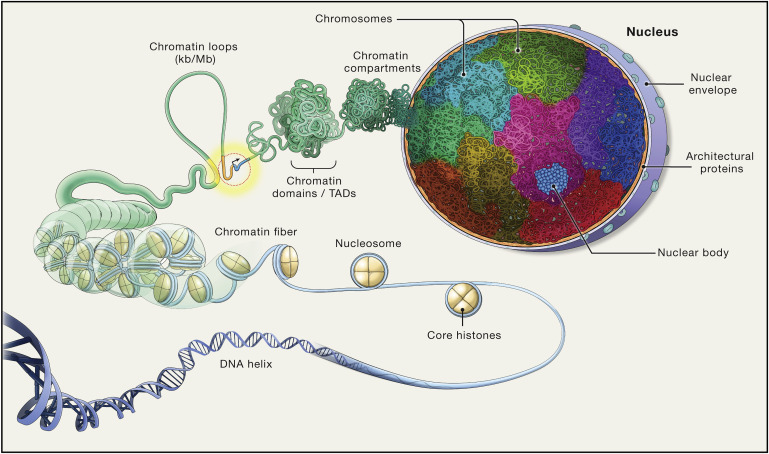
\includegraphics[width=1\textwidth]{figures/genome_organization.jpg}
    \caption[Genome organization]{\textbf{Eukaryotic genome organization.} Genomic DNA is wrapped up around histones to form nucleosomes - a basic unit of chromatin fibre. Chromatin can form loops that span kilobases (kb) or megabases (Mb) and are essential for gene expression regulation. Bigger stretches of chromatin are organized into domains or topologically associated domains (TADs), which in turn form chromatin compartments to tightly pack everything into the nucleus. Each chromosome usually occupies a territory in the nucleus. The nucleus also contains a nuclear body, architectural proteins and is surrounded by a nuclear envelope. Adapted from \cite{misteli2020self}.}
    \label{genome_organization}
\end{figure}

    \subsection{DNA}

    The existence of DNA was discovered in 1869 by Friedrich Miescher when he found a new substance inside the nuclei of the human white blood cells that did not have the same properties as proteins or lipids \cite{pray2008discovery,dahm2008discovering}. Interestingly, this is not the discovery related to DNA that is most remembered. In 1953 contributions of Rosalind Franklin, James Watson and Francis Crick led to a publication of resolved DNA molecule structure and is often considered to be the beginning of molecular biology (\colorbox{pink}{REF}). This is a fundamental moment in science history as it allowed to explain the possible mechanism of DNA replication, thus information multiplication and transfer. 

    DNA structure is based on a sugar backbone that holds four types of nucleotides - \ac{A}, \ac{T}, \ac{C} and \ac{G}.



    Deciphering DNA structure
    This provided an explanation on how proteins are encoded by genes - nucleotides in the DNA encode the amino acids in the protein chain


        \subsubsection{Types of genomic regions}
        
        A eukaryotic genome contains different types of repetitive regions or motifs. These include transposable elements, tandem repeats, GC- and AT-rich sequences, splice sites and binding sites of non-coding RNA molecules. Importantly, crucial for gene expression regulation are DNA sequence motifs targeted by transcription factors \cite{boeva2016analysis}.




    \subsection{Chromatin}


    The basic element of chromatin a 146 bp of DNA wrapped around core histone protein octamer defined as nucleosome \cite{misteli2020self}. Core histone proteins are the most commonly found in nucleosomes, but can be replaced with variants in special context, such as promoter regions.


    Types of chromatin - euchromatin and heterochromatin.



    organization of DNA into chromosome territories


    More recently, higher level organized chromatin structures are taken into account. For example, chromosome compartments.


    Phase separation maybe mention here?



